\documentclass[9pt]{IEEEtran}

\usepackage[english]{babel}
\usepackage{graphicx}
\usepackage{caption}
\captionsetup{justification=justified}

\usepackage{placeins}
\usepackage{epstopdf}
\usepackage{fancyhdr}
\usepackage{amsmath}
\usepackage{amsthm}
\usepackage{amssymb}
\usepackage{url}
\usepackage{array}
\usepackage{textcomp}
\usepackage{listings}
\usepackage{hyperref}
\usepackage{xcolor}
\usepackage{colortbl}
\usepackage{float}
\usepackage{gensymb}
\usepackage{longtable}
\usepackage{supertabular}
\usepackage{multicol}
\usepackage[justification=centering]{caption}
\usepackage{amsmath}
\usepackage{subcaption}

\usepackage[utf8x]{inputenc}

\usepackage[T1]{fontenc}
\usepackage{lmodern}
\input{glyphtounicode}
\pdfgentounicode=1

\graphicspath{{./figures/}}
\DeclareGraphicsExtensions{.pdf,.png,.jpg,.eps}

% correct bad hyphenation here
\hyphenation{op-tical net-works semi-conduc-tor trig-gs}

% ============================================================================================

\title{\vspace{0ex} Kernels and Support Vector methods}

\author{Aljaž Konec\vspace{-4.0ex}}

% ============================================================================================

\begin{document}

\maketitle

\section{Introduction}
In this report we showcase implementation of Support Vector Methods for regression tasks.
Specifically, we focus on Support Vector Regression (SVR) and Kernelized Ridge Regression (KRR).
For both methods we use the kernel trick with the Polynomial and RBF Kernels to compute encodings.



\section{Implementation: Kernelized Ridge Regression}
From normal Ridge regression, we deriver the Kernelized Ridge Regression (KRR) by replacing the dot product of $X$ and $X'$ with the kernel matrix $K$.
This gives a closed form solution for the weights $\alpha$:
$$\alpha = (K + \lambda \cdot I)^{-1} \cdot y$$
where $\lambda$ is the regularization parameter and $y$ is the target vector.


\section{Implementation: Support Vector Regression}
To find support vectors for SVR, we find the Lagrange multipliers $\alpha$ and $\alpha^*$ that maximize the dual problem:
\[
    -\frac{1}{2} \sum_{i,j=1}^n (\alpha_i - \alpha_i^*) (\alpha_j - \alpha_j^*) \langle x_i, x_j \rangle
    - \epsilon \sum_{i=1}^n (\alpha_i + \alpha_i^*)
    + \sum_{i=1}^n y_i (\alpha_i - \alpha_i^*)
\]
subject to
\[
    \sum_{i=1}^n (\alpha_i - \alpha_i^*) = 0 \quad \text{and} \quad \alpha_i, \alpha_i^* \in [0, C]
\]
Similarly to KRR, this gives us the weights $\alpha\_weight = \alpha - \alpha^*$. 

\section{Testing on synthetic sine data}
First we showcase the performance on synthetic sine data where we trained both SVR and KRR with Polynomial and RBF kernels on the entire dataset.
To find good performing hyperparameters, we used grid search for each of the methods/kernels and used best performing hyperparameters.
Figure \ref{fig:sine} shows the results of predictions using SVR and KRR with both Polynomial and RBF kernels.
Using RBF kernel for both methods approximates the sine data very well, while Polynomial kernels result in a poor fit.
The sine curve can be approximated with a Taylor expansion, but the Polynomial kernel of degree 4 is not enough to capture this expansion.
The number of support vectors for SVR with RBF kernel is 23, while for SVR with Polynomial kernel is 6.
\begin{figure}[H]
    \centering
    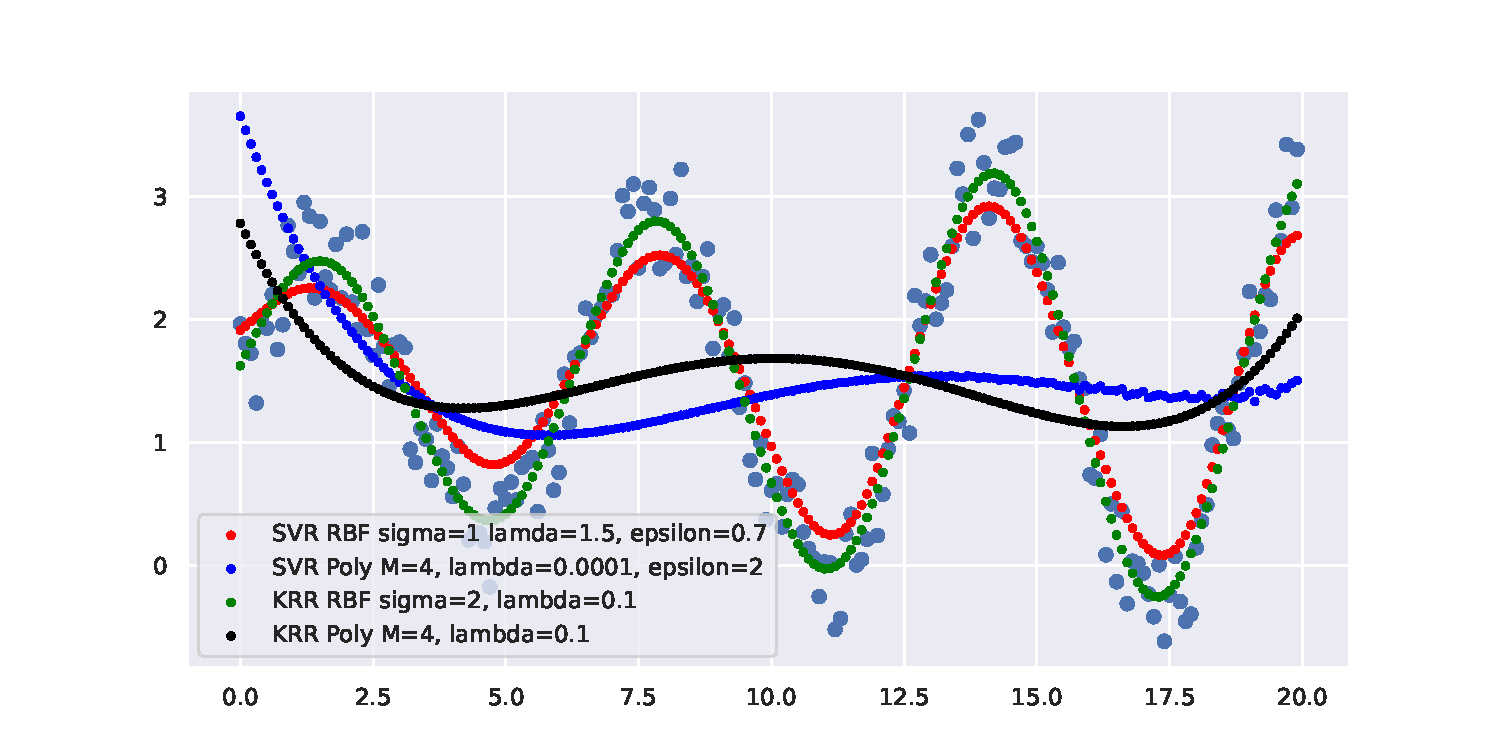
\includegraphics[width=0.55\textwidth]{sine.pdf}
    \caption{Predictions of sine data with SVR and KRR both with Polynomial and RBF kernels.}
    \label{fig:sine}
\end{figure}
For Polynomial kernels we also tried to increase the degree but that resulted in the program giving an error.
We gather that this is due to numerical instability when using higher degrees, as the kernel matrix becomes ill-conditioned.

\section{Predictions on Housing data}
Similarly to the previous homework, we used the housing data to test the performance of SVR and KRR.
For better performance, we first normalized the data.
Figure \ref{fig_housing} shows the root mean squared error (RMSE) of the predictions for both kernels with diffrent kernel parameters.
The first column represents the predicions using KRR, while the second column represents the predictions using SVR.
We show how regularization parameter $\lambda$ affects the performance of both methods.
The blue lines represent the RMSE with fixed $\lambda=1$, while the orange represent the RMSE where we use cross-validation to find the best $\lambda$ for each kernel parameter.
To find the best $\lambda$, we used GridSearchCV from sklearn with 5-fold cross-validation on the training data.
The tested $\lambda$-values were $[0.0001, 0.001, 0.01, 1, 2, 3, 4, 5, 10]$.
The parameter $\epsilon=8$ gave the best results for SVR and was kept fixed.
For SVR we also show the number of support vectors used for each kernel parameter.

Choosing a $\sigma$ that is smaller then 1 resulted in very poor performance for all tested models and lambdas.
This is due to the fact that the RBF kernel is not able to capture the complexity of the data with such a small $\sigma$ as the resulting gaussian is too narrow.
Choosing higher values for $\sigma$ did not change the performance of KRR significantly, while for SVR it resulted in a better performance.
SVR with dynamic cross-validation lambda performed better quite better than SVR with fixed lamda and achiving its minimum at $\sigma=3$.
The number of support vectors for SVR with RBF kernel also decreases if using dynamic cross-validation lambda. 
This is due to the fact that the model is able to generalize better and does not need as many support vectors to capture the complexity of the data.

\begin{figure*}[t]
    \centering
    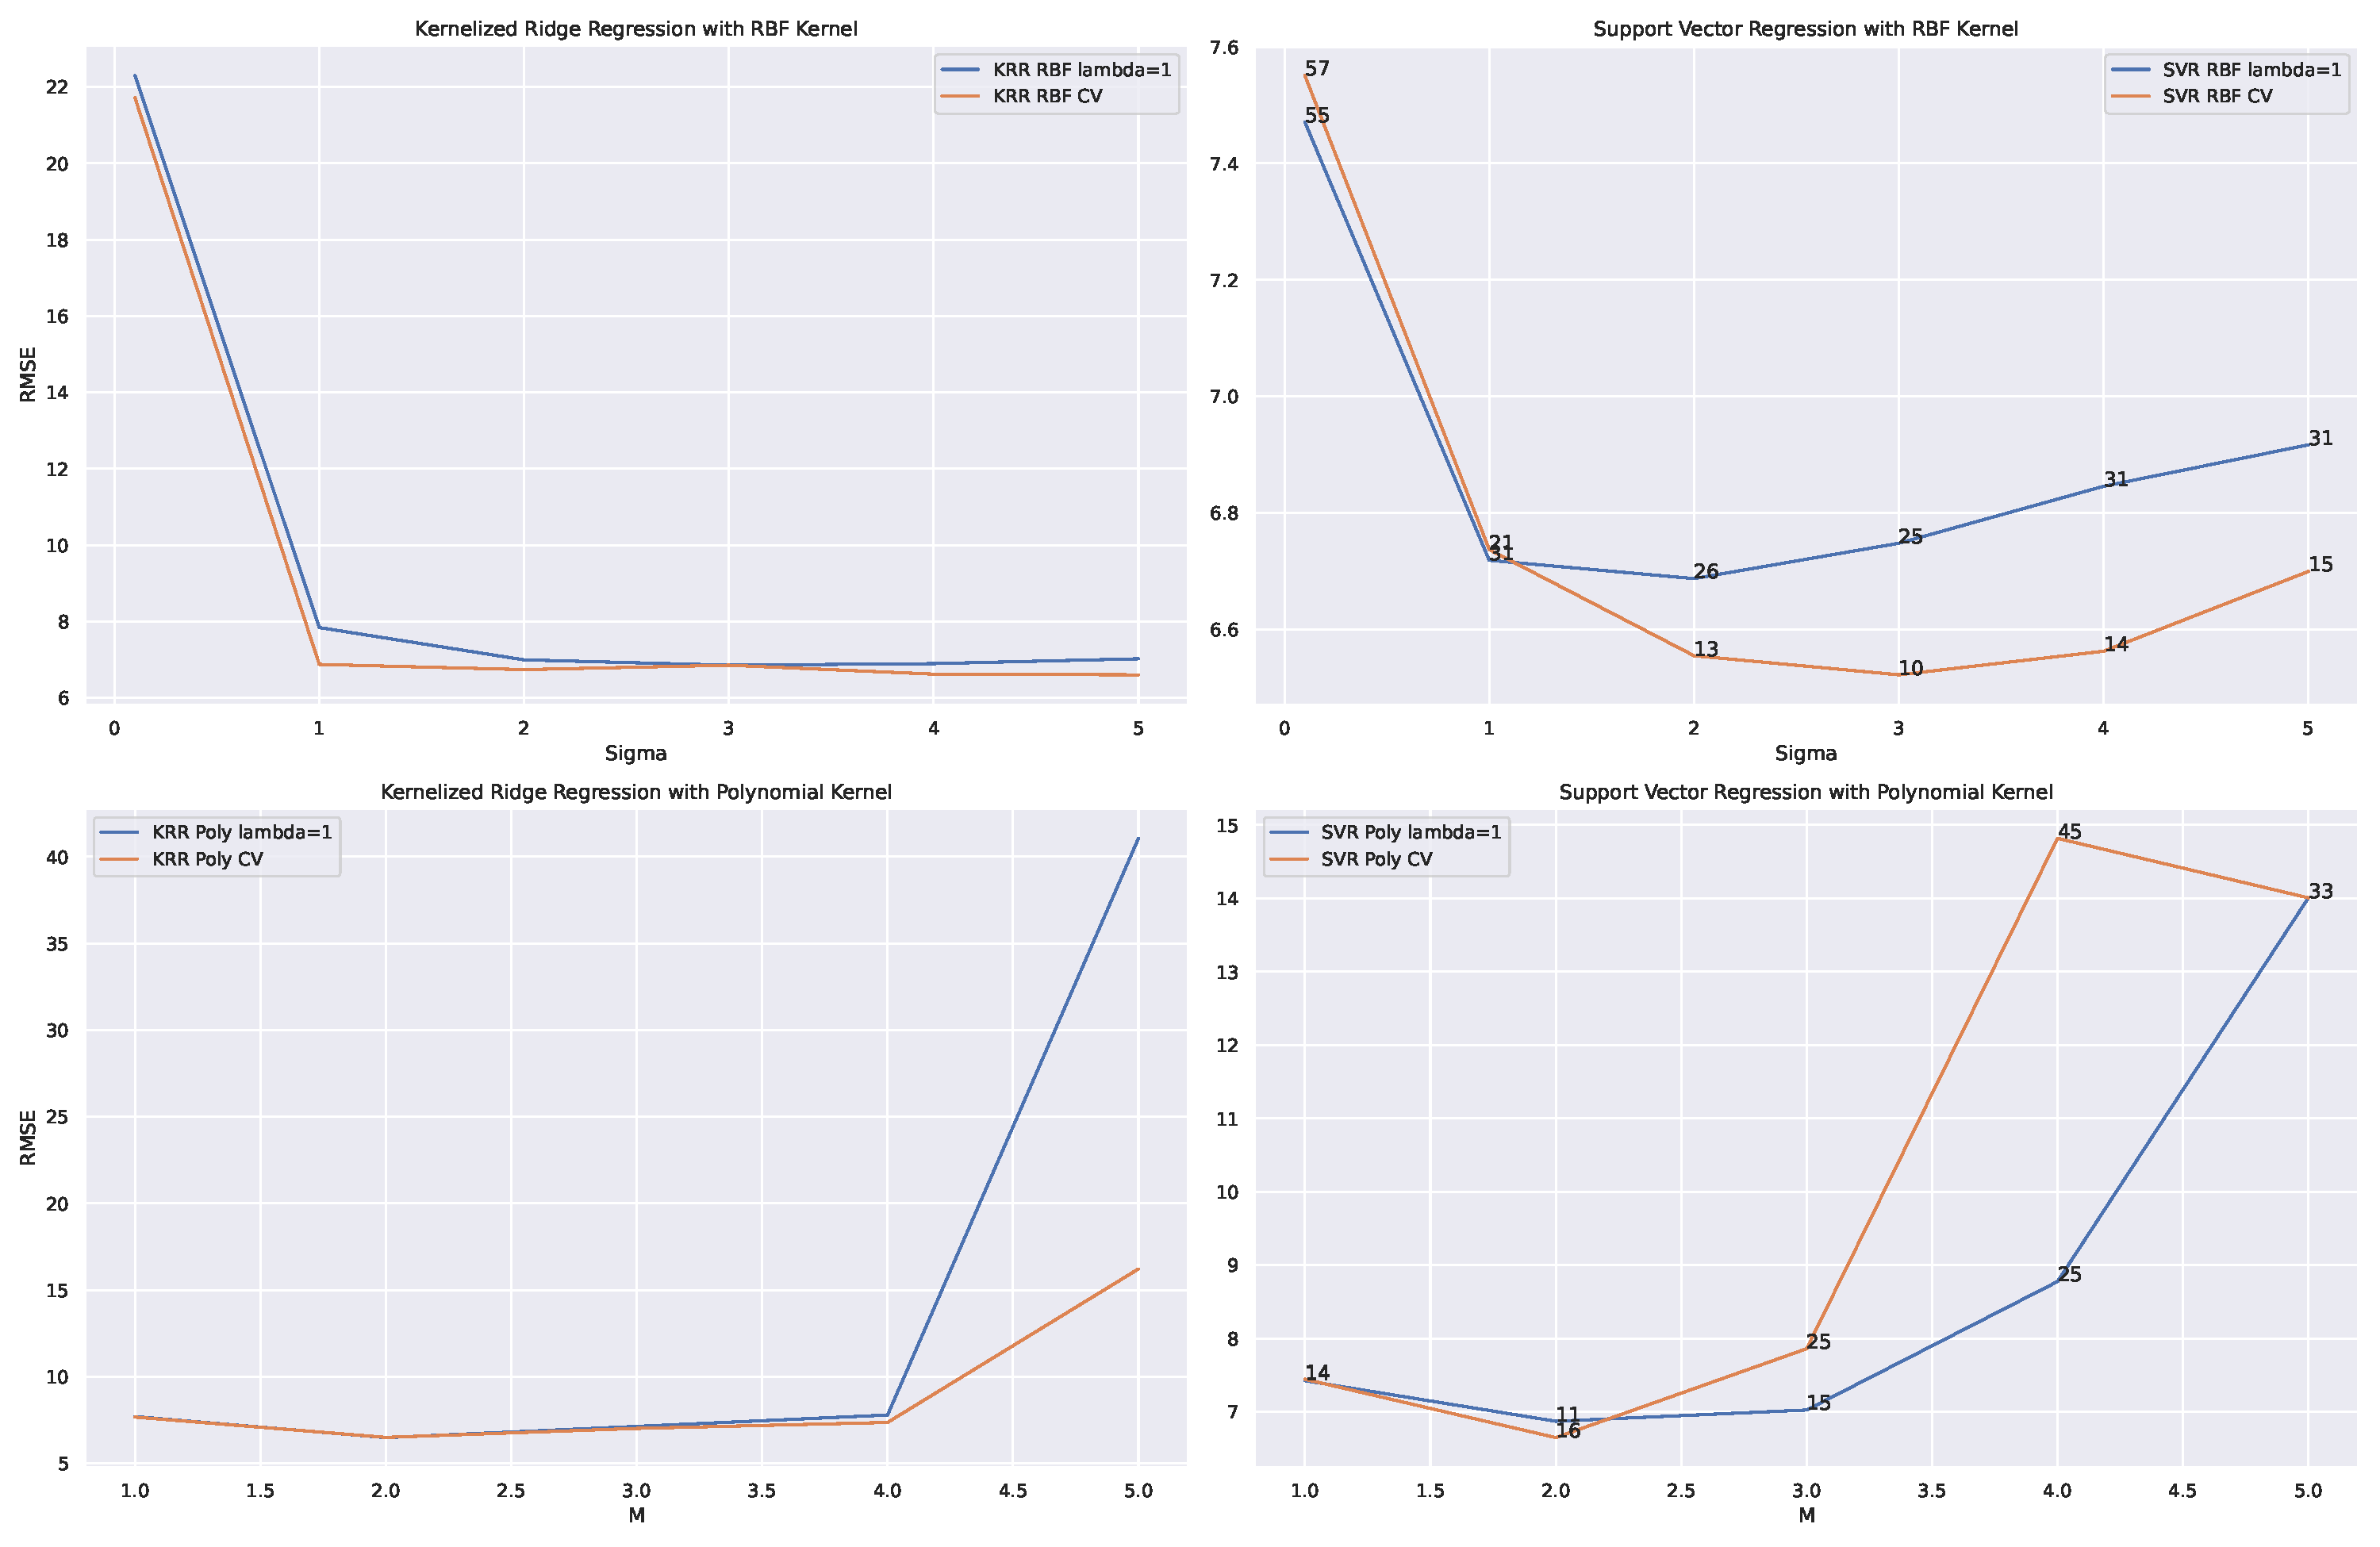
\includegraphics[width=1\textwidth]{housing_results.pdf} % dopiši še da so cifre st support vektorjev
    \caption{Predictions of housing data with SVR and KRR both with Polynomial and RBF kernels.}
    \label{fig_housing}
\end{figure*}

For Polynomial kernels we can see that increasing the degree to $M=5$ results in worse performance for both models.
This is due to the fact that the model becomes too complex and is not able to generalize well.
The number of support vectors subsequently also increases with the degree of the polynomial kernel.
Performing dynamic cross-validation lambda resulted in similar performance for KRR with an improvement in performance for $M=5$.
Interestingly, using dynamic cross-validation lambda for SVR resulted in worse performance for M largerd than 3.
Since this is a small dataset, we conclude that this is due to the lambda being overfitted to the training data.

Overall for the right choice of hyperparameters, all models and kernels achieve similar performance with RMSE between 6 and 7.
In general, using the RBF kernel resulted in slightly better and more stable performance than the Polynomial kernel.
Using dynamic cross-validation lambda resulted in better performance but might be difficult to deploy to larger datasets.



\section{Conclusion}
%Compare results between kernelized ridge regression and SVR and comment on 
%the differences and similarities. Which learning algorithm would you prefer and why?

In this report we saw that both methods are able to capture the properties of the data and achieve similar performance.
The main difference between the two methods is that SVR does not have a closed form solution and may sometimes not be a feasible optimization problem.
SVR also has a hyperparameter $\epsilon$ that needs to be taken into consideration when tuning the model.
On the other hand, KRR has a closed form solution but uses the inverse of a potentially very large kernel matrix.
Given all of this we would prefer to use SVR with RBF kernel as it offers the best performance and for larger datasets we do not need to compute the inverse of a matrix.

\section*{Conclusion}


\bibliographystyle{IEEEtran}
\bibliography{bibliography}

\end{document}
